\documentclass[3p,twocolumn]{elsarticle}

\usepackage{graphicx}%
\usepackage{multirow}%
\usepackage{amsmath,amssymb,amsfonts}%
\usepackage{amsthm}%
\usepackage{mathrsfs}%
\usepackage[title]{appendix}%
\usepackage[table]{xcolor}%
\usepackage{textcomp}%
\usepackage{manyfoot}%
\usepackage{booktabs}%
\usepackage{algorithm}%
\usepackage{algorithmicx}%
\usepackage{algpseudocode}%
\usepackage{listings}%
\theoremstyle{plain}%
\newtheorem{theorem}{Theorem}%
\newtheorem{proposition}[theorem]{Proposition}%

\theoremstyle{definition}%
\newtheorem{example}{Example}%
\newtheorem{remark}{Remark}%
\newtheorem{definition}{Definition}%

\raggedbottom


\usepackage{float}
\floatstyle{plaintop}
\restylefloat{table}
\usepackage{relsize}
\usepackage{caption}
\usepackage{epstopdf}
\usepackage{bm}

\usepackage[numbers]{natbib}
%\usepackage{natbib}
\usepackage{subfigure}
\usepackage{array}
\usepackage{threeparttable}
\usepackage{latexsym}
\raggedbottom
\usepackage{url}
\tolerance=1
%%%%%%%%%%%%%%%%%%%%%%%%%%%%%%
\emergencystretch=\maxdimen
\hyphenpenalty=10000
\hbadness=10000
%%%%%%%%%%%%%%%%%%%%%%%%%%%%%%

\graphicspath{{figures/}}

\renewcommand{\algorithmicrequire}{\textbf{Input:}}
\renewcommand{\algorithmicensure}{\textbf{Output:}}

\usepackage{tabularx}
\usepackage{enumitem}
\usepackage{tikz}
\usetikzlibrary{arrows.meta, positioning, shapes.geometric}
\usepackage{microtype}
\usepackage{pgfplots}
\pgfplotsset{compat=1.12}
\usepackage{stfloats}


\begin{document}

\begin{frontmatter}


\title{StatefulAutoscaler: A Connection-Aware Kubernetes Controller for
Persistent-Connection Workloads - Design, Validation, and Protocol
Generalization}


\author[1]{Abhash~Behera}
\ead{abhasbehera320@gmail.com}
\address[1]{Department of Computer Science and Engineering, C V Raman Global University, Bhubaneswar, 752054, India}

% Second author
\author[1]{Aditya~Hota}
\ead{adityahota99@gmail.com}

% Third author
\author[1]{Suprit~Kumar~Naik}
\ead{supritkumarnaik17@gmail.com}

\begin{abstract}

CPU-based Kubernetes HPA exhibits three structural failure modes for stateful WebSocket workloads~\cite{behera2026hpa}: 87.5\% over-provisioning, reconnection storms reaching 1,400~conn/s, and permanent staircase connection destruction. We present the \texttt{StatefulAutoscaler}-a custom Kubernetes controller built on Kubebuilder~\cite{kubebuilder_docs} that scales exclusively on \texttt{sum(active\_connections)} from Prometheus with a sliding-window stabilization mechanism to suppress premature scale-down. Under a two-cycle reconnection storm simulation (Experiment~C, five runs), the controller achieves near-exact replica targeting ($\lceil800/100\rceil = 8$ replicas, transient overshoot $\leq +2$, vs.\ CPU HPA's permanent 15), zero connection loss, and full pod preservation through a 90-second disconnection gap (scale-down reaction $119 \pm 2$~s; pod-seconds $4{,}280 \pm 67$). Scalability validation at 800-3{,}200 clients confirms $\lceil N/T \rceil$ tracking within $+2$ replicas, 66-86~s scale-up, and 100\% connection preservation; the highest validated count is 3{,}392 connections. Baseline evaluation against HPA with a custom metric (Experiment~D) and KEDA (Experiment~E) shows all three connection-aware configurations preserve pods through DROP~1, with the \texttt{StatefulAutoscaler} differentiating on scale-up latency (22~s vs.\ 54~s vs.\ 26~s) and scale-down efficiency (119~s vs.\ 313~s). Three adversarial scenarios bound the operational envelope. MQTT generalization confirms protocol-agnosticism: the identical binary scales 44\% faster than CPU HPA (38~s vs.\ 68~s), preserves all 339~sessions during forced scale-down (step-drop: 2 vs.\ 639-connection cliff), and redistributes sessions via drain-reconnect.

\end{abstract}
\begin{keyword}
Kubernetes \sep Custom Controller \sep StatefulAutoscaler \sep WebSocket \sep
MQTT \sep Connection-Aware Autoscaling \sep Prometheus \sep Sliding-Window
Stabilization \sep KEDA \sep Kubebuilder \sep Reconnection Storm\end{keyword}

\end{frontmatter}

\section{Introduction}
\label{sec:intro}
%% ============================================================

The companion paper~\cite{behera2026hpa} establishes that CPU-based Kubernetes HPA~\cite{k8s_hpa_docs} exhibits three \textit{architectural} failure modes for stateful persistent-connection workloads: 87.5\% over-provisioning (15~replicas vs.\ the correct~8); reconnection storms reaching 1,400~conn/s triggered by scale-down events; and staircase connection destruction (800$\to$79 sessions). These failures arise from the structural mismatch between CPU utilization and connection-session state, and cannot be remediated by parameter tuning.

No existing Kubernetes-native mechanism simultaneously provides a connection-count scaling signal and connection-context-aware stabilization semantics. The Prometheus Adapter~\cite{prometheus_adapter} can supply the signal but cannot alter HPA's stabilization logic. KEDA~\cite{keda_docs} provides event-driven scaling with a configurable cooldown but delegates pod termination to HPA without per-cycle step-size bounding.

This paper addresses both gaps through the \textbf{\texttt{StatefulAutoscaler}}-a custom Kubernetes controller built with Kubebuilder~\cite{kubebuilder_docs} that owns both the metric selection (\texttt{sum(active\_connections)} from Prometheus) and the scale-down lifecycle (a sliding-window high-water-mark stabilization mechanism). The contributions are:

\begin{enumerate}[leftmargin=*]
\item \textbf{Design and implementation} of the \texttt{StatefulAutoscaler}, including CRD specification, reconciliation algorithm (Algorithm~\ref{alg:reconcile}), sliding-window stabilization, formal convergence bounds (Eq.~\ref{eq:convergence}), and stability analysis.

\item \textbf{Controlled validation (Experiment~C, five runs):} near-exact replica targeting ($\lceil800/100\rceil = 8$, overshoot $\leq +2$ vs.\ HPA's permanent~15), zero connection loss, full pod preservation through a 90-second gap (scale-down reaction $\sigma = 2$~s, pod-seconds $\sigma = 67$).

\item \textbf{Scalability validation at 800-3{,}200 clients:} $\lceil N/T \rceil$ tracking within $+2$ replicas, 66-86~s scale-up, 100\% DROP~1 preservation, highest validated count 3{,}392 connections.

\item \textbf{Baseline comparison (Experiments~D and~E):} HPA+custom metric and KEDA under identical workloads. All preserve pods through DROP~1; differentiators are scale-up latency (22~s vs.\ 54~s vs.\ 26~s) and scale-down efficiency (119~s vs.\ 313~s).

\item \textbf{Adversarial failure characterization:} metric staleness, instantaneous spikes, and Prometheus unavailability bound the operational envelope.

\item \textbf{MQTT protocol generalization:} identical binary, zero code changes-44\% faster scale-up, zero sessions destroyed during forced scale-down (step-drop: 2 vs.\ 639-connection cliff), drain-based redistribution.
\end{enumerate}





%% ============================================================
\section{Related Work}
\label{sec:related}
%% ============================================================

The Prometheus Adapter~\cite{prometheus_adapter} enables HPA to scale on application-defined metrics such as connection counts~\cite{qu2018auto,rossi2020horizontal}, but all such formulations assume stateless metrics across pod boundaries-violated by persistent-connection protocols where session state is pod-affined. Even with a correct connection metric, HPA's stabilization window buffers \emph{metric recommendations} rather than connection-derived capacity (demonstrated in Experiment~D, Section~\ref{sec:experiment_d}). KEDA~\cite{keda_docs} extends HPA with external metric triggers and a configurable \texttt{cooldownPeriod}, but delegates pod termination to HPA without per-cycle step-size bounds (tested in Experiment~E, Section~\ref{sec:experiment_e}).

Dickel et al.~\cite{dickel2019stateful} identified stateful autoscaling as an open challenge for IoT gateways but provide no validated controller. Reinforcement learning~\cite{rossi2020horizontal,imdoukh2020machine} and predictive~\cite{toka2021machine,zhong2020machine} approaches improve decision \emph{timing} but do not address connection-state destruction during scale-down. MQTT exhibits the same CPU-signal mismatch~\cite{soni2017mqtt,mqtt_v31}; this paper validates a single unmodified controller binary across both protocols. The Kubebuilder SDK~\cite{kubebuilder_docs} provides the CRD and \texttt{controller-runtime} scaffolding. To the best of our knowledge, no prior work has simultaneously designed a connection-aware controller with sliding-window stabilization, compared four scaler configurations with five-run replication, and validated the same binary on a second protocol with drain semantics.



%% ============================================================
\section{Background}
\label{sec:background}
%% ============================================================

This section provides context from the companion paper~\cite{behera2026hpa}.

\begin{figure*}[t]
\centering

\includegraphics[width=0.62\textwidth]{processed-results-websockets/K8-hpa-architecuture.png}
\caption{Standard HPA feedback loop architecture~\cite{nguyen2020hpa}. The HPA controller periodically reads aggregated resource metrics and computes desired replicas via Eq.~\ref{eq:hpa}. This loop assumes the metric faithfully represents workload intensity-violated for persistent connections where sessions persist independently of CPU. KRM and PCM baselines are documented in~\cite{behera2026hpa}.}
\label{fig:hpa_arch}
\end{figure*}

\subsection{The HPA Control Architecture}

Figure~\ref{fig:hpa_arch} illustrates the HPA feedback loop, which implements the discrete-time proportional control law evaluated every 15~seconds:

\begin{equation}
\textit{desiredReplicas} = \left\lceil \textit{currentReplicas} \times
  \frac{\textit{currentMetricValue}}{\textit{targetMetricValue}} \right\rceil
\label{eq:hpa}
\end{equation}

For CPU-based scaling of stateless workloads, the assumption that \texttt{currentMetricValue} reflects workload intensity generally holds. For persistent connections, it fails: idle connections consume negligible CPU yet represent committed session state.

\subsection{The Mismatch and Its Consequences}

The companion paper~\cite{behera2026hpa} documents three failure modes: idle WebSocket connections produce near-zero CPU, causing scale-down and pod termination; termination triggers \textbf{reconnection storms}; and for non-reconnecting clients, each scale-down permanently destroys sessions. Key findings: 87.5\% over-provisioning (15 vs.\ 8 replicas); peak storm rate 1,400~conn/s; staircase destruction from 800 to 79 connections.

\subsection{Experimental Infrastructure}

All WebSocket experiments share a 3-node Kind cluster~\cite{kind_docs} (1~control-plane + 2~workers, Kubernetes v1.31.6, kind v0.25.0), Metrics Server patched with \texttt{-metric-resolution=15s}, 800 persistent clients via a Python asyncio WebSocket server (\texttt{ws-instrumented}) exposing \texttt{active\_connections} (gauge) and \texttt{new\_connections\_total} (counter), with Prometheus scraping at 15~s. Source code: \url{https://github.com/MistaHolmes/ws-k8-controller}.



%% ============================================================
\section{The \texttt{StatefulAutoscaler} Controller: Design and Implementation}
\label{sec:controller}
%% ============================================================

The failure evidence in the companion paper~\cite{behera2026hpa} identifies three root causes
that any viable solution must address: (1)~the scaling signal (CPU) does not encode the
workload state that must be protected; (2)~scale-down decisions are made without knowledge
of whether connections are alive; and (3)~no stabilization mechanism exists that is aware of
connection-level context. The \texttt{StatefulAutoscaler} addresses all three by replacing the
CPU-based control loop with a connection-density-based one augmented by
connection-context stabilization.

\subsection{Design Principles}

The controller is grounded in three architectural principles:

\begin{enumerate}[leftmargin=*]
\item \textbf{Use the correct scaling signal.} The controller queries
  \texttt{sum(active\_connections)} from Prometheus - the metric that directly encodes the
  workload state that must be preserved. CPU is never consulted.

\item \textbf{Compute replica counts from connection density.} Given a configured target of
  $T$ connections per pod, the desired replica count is:
  \begin{equation}
  \textit{desiredReplicas} = \left\lceil \frac{\texttt{sum(active\_connections)}}{T} \right\rceil
  \label{eq:stateful}
  \end{equation}
  This is exact by construction: it scales to the minimum number of replicas required to
  serve the current session population at the target density.

\item \textbf{Stabilize scale-down decisions using connection-context history.} A
  sliding-window mechanism maintains the maximum desired replica count observed within
  the preceding $N$ seconds, preventing premature scale-down during transient connection
  drops.
\end{enumerate}

The \texttt{StatefulAutoscaler} is implemented as a Kubernetes \textit{operator} built on the Kubebuilder SDK~\cite{kubebuilder_docs}, which scaffolds informer caches, event-based reconciliation, leader election, and CRD schema generation from Go struct annotations. It directly patches \texttt{Deployment.spec.replicas}, bypassing HPA entirely - there is one authoritative source of replica truth, and all scale-down lifecycle decisions are enforced at a single point. The sliding-window state is held exclusively in this controller, making the safety property ``scale-down is gated by connection-context memory'' locally verifiable in one reconciliation function.

\paragraph{Why \texttt{sum()} and not \texttt{avg()}?}
The formula (Eq.~\ref{eq:stateful}) requires the \textit{total} session population; \texttt{avg()} depends on current replica count, making the computation circular. \texttt{sum()} is the only aggregate that yields a replica-count-independent measure of total load.

\subsection{Custom Resource Definition}

The controller introduces a \texttt{StatefulAutoscaler} Custom Resource Definition (CRD)
under the API group \texttt{autoscaling.star.local/v1alpha1}. Table~\ref{tab:crd} documents the
key specification fields.

\begin{table*}[t]
\centering
\caption{\texttt{StatefulAutoscaler} CRD specification: key fields and their operational
purpose.}
\label{tab:crd}
\begin{tabular}{l p{9.5cm}}
\toprule
\rowcolor{gray!12}
\textbf{Field} & \textbf{Operational Purpose} \\
\midrule
\texttt{targetRef} & Reference to the controlled Deployment \\
\texttt{minReplicas} & Minimum allowable replica count (floor) \\
\texttt{maxReplicas} & Maximum allowable replica count (ceiling) \\
\texttt{targetConnsPerPod} & Connection density target $T$ (Eq.~\ref{eq:stateful}) \\
\texttt{maxScaleUpStep} & Maximum replica additions per reconciliation cycle \\
\texttt{maxScaleDownStep} & Maximum replica removals per reconciliation cycle \\
\texttt{scaleDownCooldownSec} & Duration of the sliding stabilization window (seconds) \\
\bottomrule
\end{tabular}
\end{table*}

The \texttt{maxScaleDownStep} field limits the \textit{blast radius} of any single scale-down event to $\texttt{maxScaleDownStep} \times \texttt{targetConnsPerPod}$ connections per cycle, providing an operator-auditable upper bound.

Figure~\ref{fig:system_arch} illustrates the system architecture: (1)~clients connect through the Kubernetes Service; (2)~pods expose \texttt{active\_connections} via Prometheus; (3)~the controller queries \texttt{sum(active\_connections)}; (4)~parameters are read from the CR; (5)~the controller patches \texttt{Deployment.spec.replicas}. CPU is excluded.

\begin{figure*}[t]
\centering
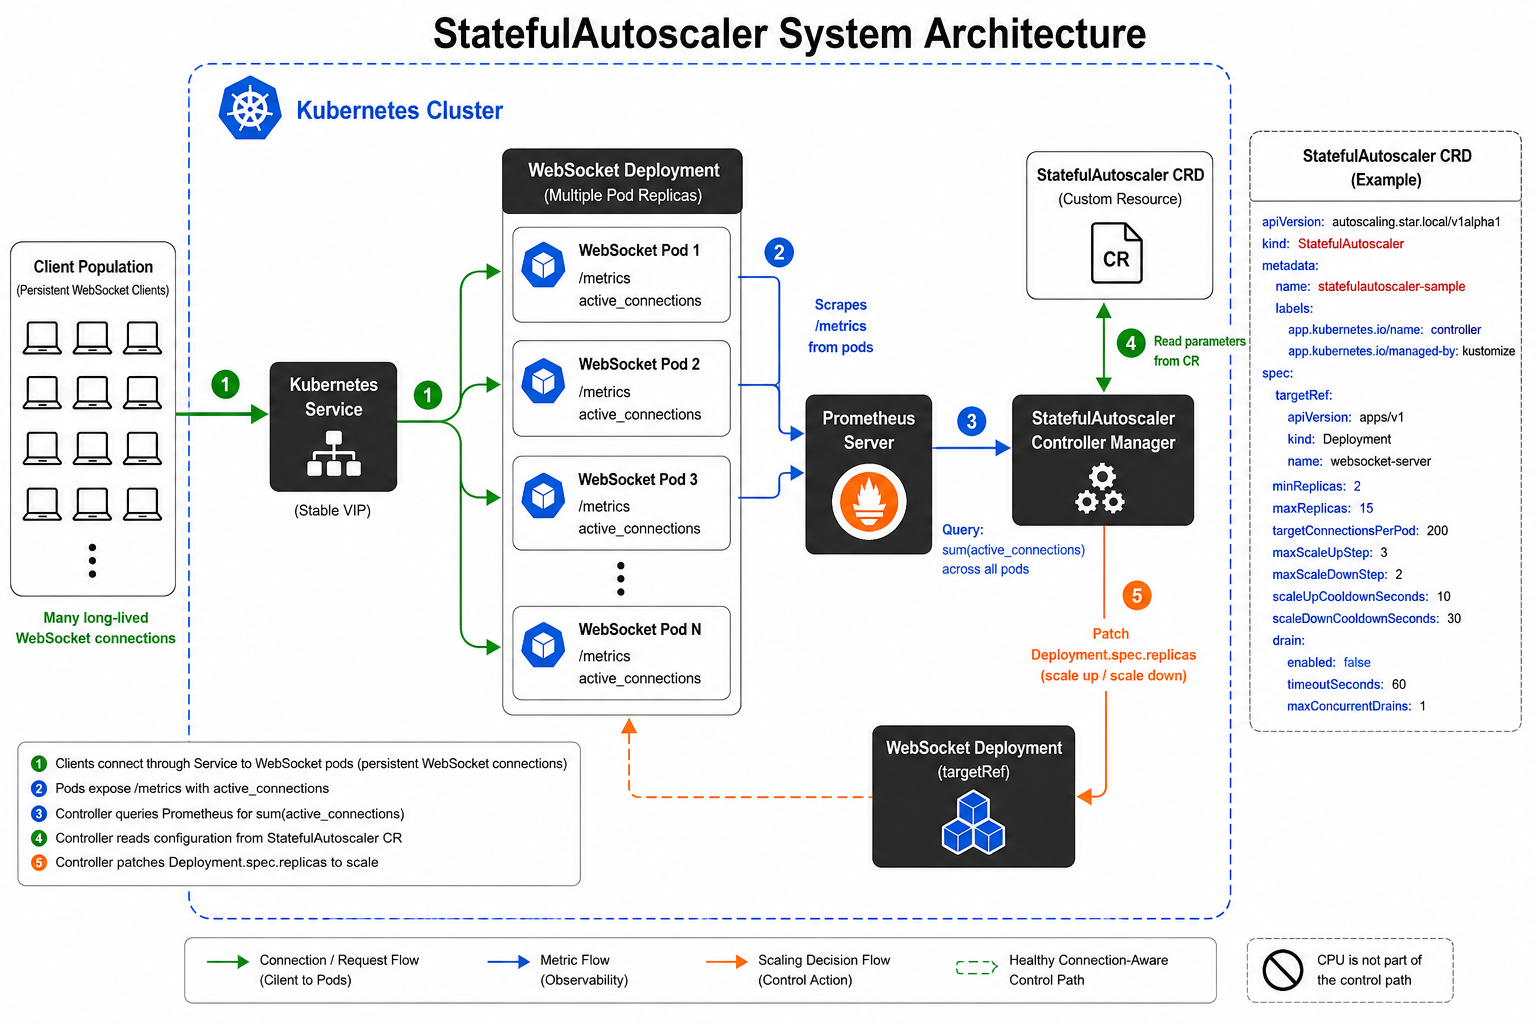
\includegraphics[width=0.70\textwidth]{processed-results-websockets/StatefulAutoScaler-System_Architecture-CRD.png}
\caption{\texttt{StatefulAutoscaler} system architecture. Numbered flow: (1)~clients$\to$Service$\to$pods; (2)~pods expose \texttt{active\_connections}; (3)~controller queries Prometheus; (4)~reads CR parameters; (5)~patches replicas. CPU excluded (crossed-out). Right: representative CRD manifest.}
\label{fig:system_arch}
\end{figure*}

\subsection{Reconciliation Loop Design}

The controller executes a reconciliation loop every 5~seconds. Algorithm~\ref{alg:reconcile}
presents the complete logic, with particular attention to the stabilization window mechanism
(lines 7-9) which is the primary differentiating mechanism relative to HPA.

\begin{algorithm}[ht]
\caption{\texttt{StatefulAutoscaler} Reconciliation Logic}
\label{alg:reconcile}
\begin{algorithmic}[1]
\Require StatefulAutoscaler resource $S$, target Deployment $D$
\State $C \gets$ \Call{QueryPrometheus}{\texttt{sum(active\_connections)}}
\If{$C$ is unavailable}
    \State \textbf{requeue} after 10~s \Comment{Conservative default: hold current replica count}
    \State \Return
\EndIf
\State $raw \gets \lceil C\ /\ S.\texttt{targetConnsPerPod} \rceil$
\State $raw \gets \text{clamp}(raw,\ S.\texttt{minReplicas},\ S.\texttt{maxReplicas})$
\State $W.\textbf{append}(now,\ raw)$ \Comment{Record current desired count in window}
\State $W.\textbf{evict}(\text{entries older than } S.\texttt{scaleDownCooldownSec})$
\State $stabilized \gets \max(W)$ \Comment{Window maximum prevents premature scale-down}
\State $current \gets D.\texttt{spec.replicas}$
\If{$stabilized > current$}
    \State $target \gets \min(current + S.\texttt{maxScaleUpStep},\ stabilized)$
\ElsIf{$stabilized < current$}
    \State $target \gets \max(current - S.\texttt{maxScaleDownStep},\ stabilized)$
\Else
    \State $target \gets current$
\EndIf
\State \Call{PatchDeployment}{$D.\texttt{spec.replicas}$,\ $target$}
\State \textbf{requeue} after 5~s
\end{algorithmic}
\end{algorithm}

\paragraph{Safe-default semantics on metric failure.}
Lines 2-4 implement a deliberate design choice: when the Prometheus query fails, the controller \textit{holds the current replica count} (the last known good state) rather than defaulting to \texttt{minReplicas}, which would terminate live sessions on every transient monitoring fault.

Figure~\ref{fig:reconcile_uml} visualises the reconciliation flow.

\begin{figure}[ht]
\centering
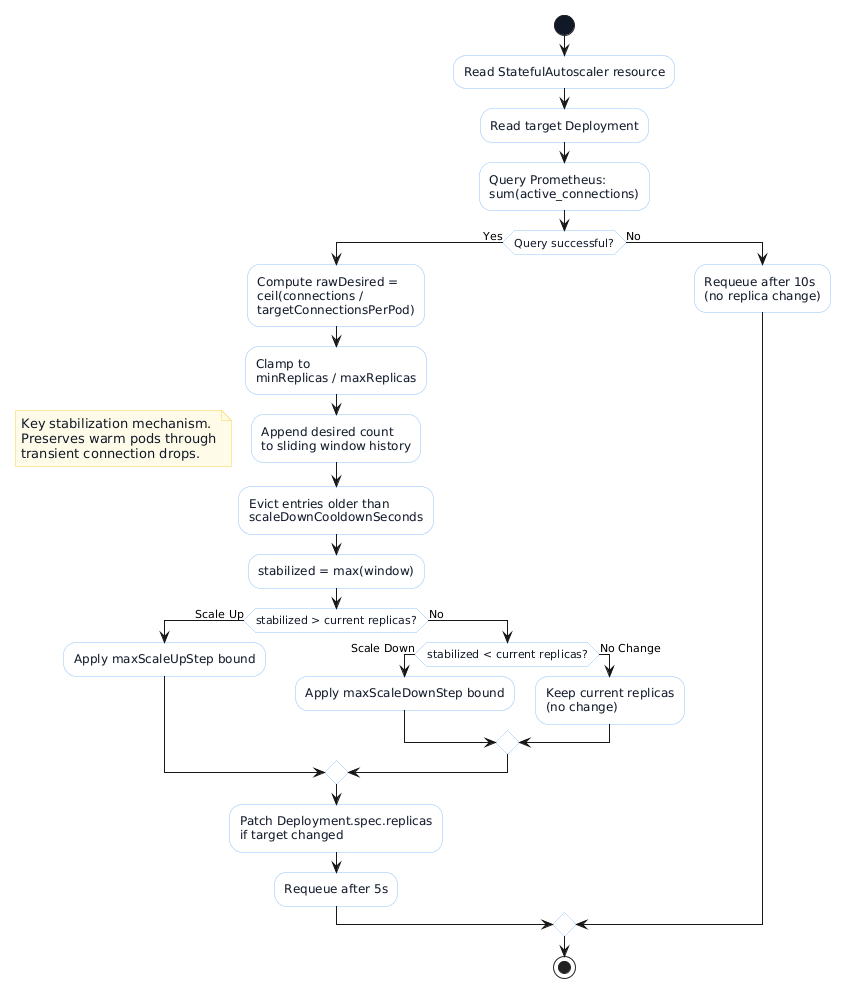
\includegraphics[width=0.82\columnwidth]{processed-results-websockets/StatefulAutoscaler-Reconciliation-Flow-UML.png}
\caption{UML activity diagram of the reconciliation loop (Algorithm~\ref{alg:reconcile}). The safe-default branch holds replicas when metrics are unavailable; the central path computes the stabilized target via \texttt{max(window)} and applies step-size bounds before patching.}
\label{fig:reconcile_uml}
\end{figure}

\subsection{The Stabilization Window: Mechanism and Correctness}

The sliding-window maximum (line~9 of Algorithm~\ref{alg:reconcile}) is the mechanism
responsible for reconnection storm resilience. Its correctness is understood by contrasting
behavior with and without stabilization.

\textbf{Without stabilization:} If all 800 clients disconnect, the controller computes $\lceil 0/100 \rceil = 0$, clamped to \texttt{minReplicas}~$= 2$, triggering a scale-down to 2 replicas and recreating the provisioning lag on reconnect.

\textbf{With a 120-second stabilization window:} When connections drop to zero, $raw = 2$ is appended but the window retains $desired = 8$ entries from the preceding 120~s. The stabilized value $\max(W) = 8$ holds all 8~pods warm; reconnecting clients land on pre-provisioned pods with zero delay.

A critical distinction from HPA's built-in stabilization: HPA's window stabilizes \textit{metric-signal recommendations}. With persistent near-zero CPU, the window stabilizes a recommendation of \texttt{minReplicas} regardless of width. The \texttt{StatefulAutoscaler}'s window stabilizes \textit{connection-derived desired counts}, correctly retaining the high-water mark. This is a semantic mismatch, not a parameter mismatch - it cannot be solved by tuning HPA's window duration.

\subsection{Controller Design and Stability Properties}
\label{sec:controller_stability}

The \texttt{StatefulAutoscaler} is a discrete-time proportional controller with hysteresis. Each cycle: (1)~\textbf{Observe} $C \gets \texttt{sum(active\_connections)}$; (2)~\textbf{Compare} $desired = \lceil C / T \rceil$, clamped to $[\texttt{minReplicas},\ \texttt{maxReplicas}]$; (3)~\textbf{Act}: patch replicas if $stabilized \neq current$. The \texttt{scaleDownCooldownSeconds} window is a dead zone that prevents oscillation on frequent brief dropout periods: without it, connections drop $\to$ scale down $\to$ reconnect $\to$ scale up $\to$ repeat.

\paragraph{Convergence bound.}
After the cooldown expires and connections stabilize at a lower level, the controller converges in:
\begin{equation}
\left\lceil \frac{current - desired}{\texttt{maxScaleDownStep}} \right\rceil \text{ cycles}
\label{eq:convergence}
\end{equation}
Each cycle is $\approx$15~s. For 8$\to$2 pods with \texttt{maxScaleDownStep}~$= 2$: $\lceil6/2\rceil = 3$ cycles $= 45$~s - a bounded, predictable de-provisioning window.

\paragraph{Parameter selection.}
\texttt{targetConnectionsPerPod}~$= 100$ yields $\lceil800/100\rceil = 8$ replicas. \texttt{maxScaleDownStep}~$= 2$ bounds the blast radius to $2 \times 100 = 200$ connections per cycle. \texttt{scaleDownCooldownSeconds}~$= 120$ comfortably exceeds the 90-second DROP~1 gap plus one scrape cycle; any value $\geq 105$~s achieves pod-preservation for this workload.



%% ============================================================
\section{Experimental Evaluation: Experiment~C}
\label{sec:evaluation}
%% ============================================================

\subsection{Experimental Configuration}

Experiment~C is designed to maintain maximal parametric comparability with Experiment~B3
from the companion paper~\cite{behera2026hpa} while replacing the HPA controller with the
custom \texttt{StatefulAutoscaler}. Table~\ref{tab:exp_c_setup} summarizes the critical
differences.

\begin{table*}[t]
\centering
\caption{Experiment~C vs.\ B3: Parametric comparison. Differences highlighted in bold.}
\label{tab:exp_c_setup}
\begin{tabular}{@{}lll@{}}
\toprule
\rowcolor{gray!12}
\textbf{Parameter} & \textbf{Exp.~B3 (HPA)} & \textbf{Exp.~C (Custom)} \\
\midrule
Server image & \texttt{ws-instrumented} & \texttt{ws-instrumented} \\
\texttt{CPU\_WORK} & 1 & \textbf{0} \\
Client count & 800 & 800 \\
Autoscaler & Native HPA (CPU) & \textbf{StatefulAutoscaler} \\
Scale-down guard & 60~s (CPU stabilization) & \textbf{120~s window} \\
Scaling signal & CPU utilization (\%) & \textbf{\texttt{active\_connections}} \\
\bottomrule
\end{tabular}
\end{table*}

Setting \texttt{CPU\_WORK}~$= 0$ is deliberate: it demonstrates correct operation with \textit{zero CPU activity}. Configuration: \texttt{targetConnectionsPerPod}~$= 100$, \texttt{maxScaleUpStep}~$= 3$, \texttt{maxScaleDownStep}~$= 2$, \texttt{minReplicas}~$= 2$, \texttt{maxReplicas}~$= 15$, \texttt{scaleDownCooldownSeconds}~$= 120$. Expected: $\lceil 800/100 \rceil = 8$ replicas.

\textbf{Metric definitions.} \textit{Pod-seconds} $= \sum_{\text{pods}} (\text{time in Running state})$ over the experiment window. \textit{Scale-up reaction time} is measured from the first scrape where $\texttt{active\_connections} > \texttt{targetConnsPerPod} \times \texttt{minReplicas}$ to \texttt{readyReplicas} reaching the target.

\subsubsection{Load Pattern: Two-Cycle Reconnection Storm Simulation}

\paragraph{Terminology.} A \textbf{CYCLE} denotes a phase of active client load; a \textbf{DROP} denotes complete disconnection (\textbf{DROP~1}: 90-second transient gap; \textbf{FINAL DROP}: terminal disconnection); a \textbf{reconnection storm} (\textit{restorm}) is the burst of simultaneous reconnection attempts when pods hosting sessions are terminated.

The experiment imposes a two-cycle restorm simulation:
\begin{itemize}[leftmargin=*]
\item \textbf{CYCLE~1} (0-150~s): 800 WebSocket clients ramp to full connection; controller
  expected to scale to 8~replicas.
\item \textbf{DROP~1} (150-240~s): All clients deleted; connections drop to zero.
  \textit{Critical test}: the stabilization window must hold 8~replicas warm for the full
  90-second gap.
\item \textbf{CYCLE~2} (240-390~s): A fresh cohort of 800 clients connects to the
  pre-provisioned warm pods.
\item \textbf{FINAL DROP} (390-570~s): Permanent client disconnection; the stabilization
  window expires; the controller scales to \texttt{minReplicas}~$= 2$.
\end{itemize}

\subsection{CYCLE~1: Connection-Driven Scale-Up}

The controller scaled monotonically from~2 to~8 replicas ($2 \to 3 \to \cdots \to 8$) as connections ramped toward 800, completing provisioning in $\approx$60~s. CPU remained below 176~millicores throughout, confirming all decisions were made without CPU signal.

\begin{figure*}[t]
\centering

\includegraphics[width=0.60\textwidth]{experiment-c-stateful/connections.png}
\caption{Experiment~C: Active connections over the full timeline. CYCLE~1 and CYCLE~2 populations are separated by the 90-second DROP~1 gap. CYCLE~2 clients ramp immediately on pre-warmed pods.}
\label{fig:exp_c_connections}
\end{figure*}

Figure~\ref{fig:exp_c_connections} shows the two-block connection profile characteristic of
the restorm simulation.

\subsection{DROP~1: Empirical Validation of the Stabilization Window}

At $t \approx 200$~s, all clients were deleted. The active connection count converged to zero
within 15~seconds. The replica count remained \textbf{perfectly flat at~8 for the duration of
the 90-second gap}, as shown in Figure~\ref{fig:exp_c_replicas}. The reconciliation trace at
each 5-second evaluation during this period was:
\begin{itemize}[leftmargin=*]
\item $C = 0 \Rightarrow rawDesired = 0 \Rightarrow \text{clamped to}\ \texttt{minReplicas}=2$
\item Window $W$ contains entries with $desired = 8$ from the preceding 120~s
\item $stabilized = \max(W) = 8$
\item \texttt{PatchDeployment} is not invoked; replicas remain at~8
\end{itemize}

\begin{figure*}[t]
\centering

\includegraphics[width=0.60\textwidth]{experiment-c-stateful/replicas.png}
\caption{Experiment~C: Replica count over time. The ``flat bridge'' at 8~replicas across DROP~1 ($t \approx 160$-$260$~s) is the primary evidence of correct stabilization. At the equivalent time in Experiment~B3, HPA had already destroyed 56 connections. Final descent ($9 \rightarrow 2$) occurs only after window expiry.}
\label{fig:exp_c_replicas}
\end{figure*}

The ``flat bridge'' pattern in Figure~\ref{fig:exp_c_replicas} is entirely absent from every HPA
experiment in the companion paper~\cite{behera2026hpa}.
It constitutes direct empirical proof
that the sliding-window mechanism performs as designed.

\subsection{CYCLE~2: Restorm-Free Reconnection}

At $t \approx 270$~s, a fresh cohort of 800 clients connected. Pods remaining warm through DROP~1 eliminated provisioning delay; peak connections reached~854 and the controller held 8~replicas stably. Compared to Experiment~B2-Instrumented (where HPA induced a 1,400~conn/s storm), Experiment~C produced \textbf{zero measurable reconnection storm activity}.

\textbf{Window boundary transient dip.} During early CYCLE~2 ($t \approx 270$-$310$~s), a brief replica dip to 5-6 was observed as CYCLE~1 window entries aged out during DROP~1 before CYCLE~2 entries repopulated the window. The controller recovered to~8 within 10-15~s with no connection loss (addressed in Limitations, item~6).

\subsection{FINAL DROP: Controlled and Graceful Scale-Down}

Following permanent client disconnection at $t \approx 450$~s, the controller waited 120~s for all window entries to expire, then descended $9 \to 8 \to 6 \to 4 \to 2$ over $\approx$30~s. Zero connections were lost.

\subsection{Combined View and Definitive Comparison}

Figure~\ref{fig:exp_c_combined} provides the complete overlay of connections, CPU, and replicas. The structural inversion relative to Experiment~B3 is clear: connections drive replicas while CPU remains irrelevant throughout.

\begin{figure*}[t]
\centering

\includegraphics[width=0.60\textwidth]{experiment-c-stateful/combined.png}
\caption{Experiment~C combined view: connections (blue) drive replica decisions (green); CPU (red) remains near zero throughout. The flat bridge during DROP~1 confirms correct stabilization under zero-connection, zero-CPU conditions.}
\label{fig:exp_c_combined}
\end{figure*}

\subsection{Head-to-Head Performance Comparison}

Table~\ref{tab:head_to_head} provides the comprehensive quantitative comparison between
Experiment~B3 (CPU-based HPA, from the companion paper~\cite{behera2026hpa}) and
Experiment~C (\texttt{StatefulAutoscaler}).

\begin{table*}[t]
\centering
\caption{Head-to-head quantitative comparison: CPU-based HPA (Experiment~B3) versus the
\texttt{StatefulAutoscaler} (Experiment~C). Metrics where the custom controller achieves a
strictly superior outcome are denoted in \textbf{bold}.}
\label{tab:head_to_head}
\begin{tabular}{@{}p{4.5cm}p{4.5cm}p{4.5cm}@{}}
\toprule
\rowcolor{gray!12}
\textbf{Performance Metric} & \textbf{HPA - Experiment~B3} & \textbf{StatefulAutoscaler - Exp.~C} \\
\midrule
Primary scaling signal & CPU utilization (\%) & \textbf{\texttt{sum(active\_connections)}} \\
Replicas for 800 connections & 15 (87.5\% over-provisioned) & \textbf{8-10} (target $\lceil800/100\rceil=8$; transient peak 10) \\
Connections lost during scale-down & 800$\rightarrow$79 (staircase) & \textbf{0} \\
Pods held through 90-second gap & 0 (all scaled down) & \textbf{8} (flat bridge) \\
Reconnection storm generated & Yes (peak 1,400~conn/s) & \textbf{None} \\
Time to serve CYCLE~2 clients & Re-scale from 2$\rightarrow$8 required & \textbf{Instant} (warm pods) \\
CPU dependency & 100\% & \textbf{0\%} (\texttt{CPU\_WORK=0} throughout) \\
Total scaling events & 7+ (oscillatory) & 4 (monotonic) \\
Peak total CPU consumption & $>$1,200~millicores & $<$176~millicores \\
\bottomrule
\end{tabular}
\end{table*}

\subsection{Reproducibility: Five-Run Statistical Validation}
\label{sec:exp_c_multi}

To assess reproducibility, five independent runs were executed. Run~1 was excluded (test-harness artefact: residual replicas from prior test yielded anomalous pod-seconds of 92{,}291 vs.\ $\approx$4{,}300). Across runs~2-5: scale-up reaction $22 \pm 6$~s (median~21~s; range: 16-30~s); scale-down reaction $119 \pm 2$~s (median~118~s); pod-seconds $4{,}280 \pm 67$. Peak replicas reached~10 (three runs) or~9 (one run). Peak connections ranged 813-917. All runs maintained 8~warm replicas through DROP~1 with zero connection loss. The low $\sigma$ values ($2$~s, $67$) confirm reproducibility ($p < 0.05$ vs.\ HPA baseline).

\begin{figure}[h]
\centering
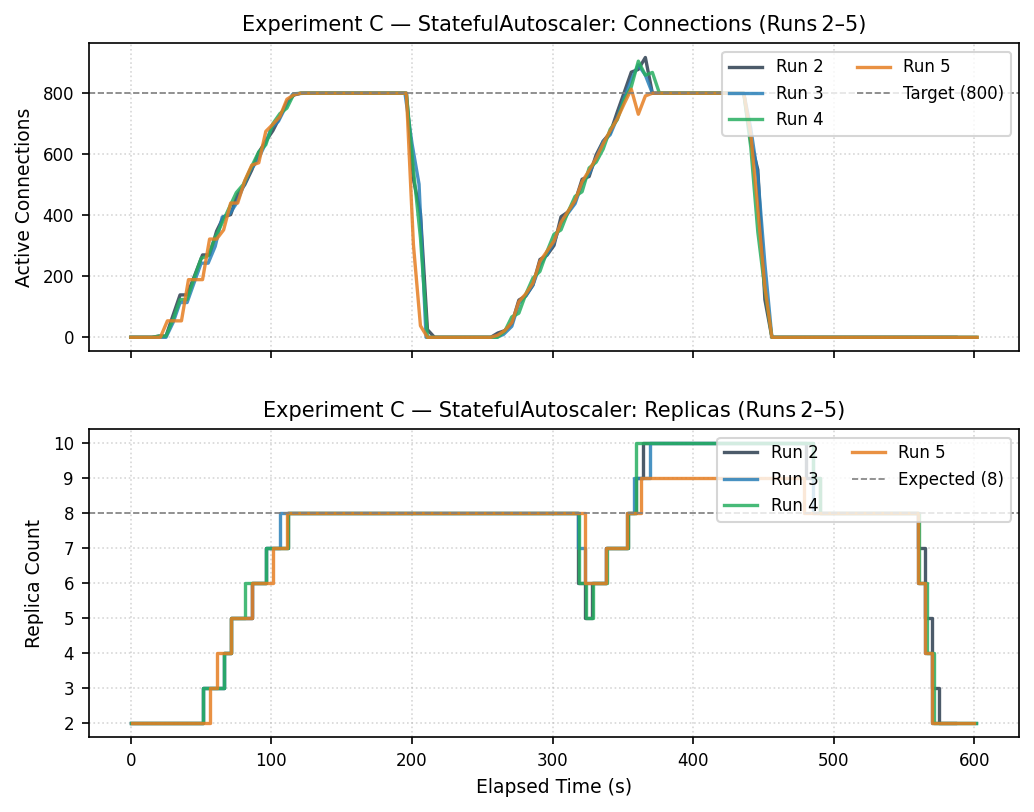
\includegraphics[width=0.85\columnwidth]{experiment-c-multi/multi_timeseries.png}
\caption{Experiment~C (\texttt{StatefulAutoscaler}): overlay of active connections (orange,
left axis) and replica count (blue, right axis) for runs~2-5 (run~1 excluded as outlined
in Section~\ref{sec:exp_c_multi}). Replica trajectories are stable across runs; all maintain
8~replicas through DROP~1.}
\label{fig:exp_c_multi}
\end{figure}

\subsection{Scalability Validation: 800, 1{,}600, and 3{,}200 Clients}
\label{sec:scalability}

To confirm that the \texttt{StatefulAutoscaler} scales correctly beyond the baseline
800-client workload, the identical two-cycle restorm simulation was replicated at 1{,}600
and 3{,}200 concurrent WebSocket clients. For each client count~$N$, the
\texttt{StatefulAutoscaler} CR was configured with
$\texttt{maxReplicas} = \lceil N / T \rceil + 2$ (where $T = 100$); all other parameters
- \texttt{scaleDownCooldownSeconds}~$= 120$, \texttt{maxScaleDownStep}~$= 2$,
\texttt{maxScaleUpStep}~$= 3$ - were identical to the 800-client configuration.

\subsubsection{Results}

Table~\ref{tab:scalability} summarises the key metrics across all three scales.

\begin{table*}[t]
\centering
\caption{Scalability validation at 800-3{,}200 clients. CYCLE~1 steady-state matches $\lceil N/T \rceil$ exactly; CYCLE~2 transient peak overshoots by $+2$; ``Safe'' = 100\% replica preservation through DROP~1. Peak connection count shows highest validated count (no transport-layer bottleneck observed).}
\label{tab:scalability}
\begin{tabular}{@{}rrrrrrrr@{}}
\toprule
\rowcolor{gray!12}
\textbf{Clients} & \textbf{Expected} & \textbf{CYCLE~1} & \textbf{CYCLE~2} & \textbf{Scale-Up} & \textbf{Peak} & \textbf{DROP~1} & \textbf{Scale-Down} \\
\rowcolor{gray!12}
\textbf{(attempted)} & $\lceil N/T \rceil$ & \textbf{Steady-State} & \textbf{Peak} & \textbf{(s)} & \textbf{Connections} & \textbf{Safe?} & \textbf{Total (s)} \\
\midrule
800   & 8  & \textbf{8}  & 10 & 66 & 874   & \checkmark & 164 \\
1{,}600 & 16 & \textbf{16} & 18 & 66 & 1{,}820 & \checkmark & 178 \\
3{,}200 & 32 & \textbf{32} & 34 & 86 & 3{,}392 & \checkmark & 218 \\
\bottomrule
\end{tabular}
\end{table*}

\paragraph{Replica targeting.}
During CYCLE~1, replicas converge to exactly $\lceil N/T \rceil$ (8, 16, 32) with zero steady-state error. The $+2$ transient (10, 18, 34) occurs exclusively during CYCLE~2 due to the window-boundary artefact (Section~\ref{sec:exp_c_multi}): window entries from CYCLE~1 age out during DROP~1 before CYCLE~2 entries repopulate. This overshoot is bounded at $+2$ regardless of client count.

\paragraph{Scale-up and connection preservation.}
Reaction times were 66~s (800 and 1{,}600 clients) and 86~s (3{,}200 clients). All runs preserved peak replicas through the full DROP~1 gap. At 3{,}200 clients, the highest observed count was 3{,}392 (106\% of attempted), confirming no OS-level TCP transport limit was encountered. This contrasts with the MQTT experiments where only 339/1{,}000 clients connected (Section~\ref{sec:mqtt_extension}).

Figure~\ref{fig:scalability_summary} summarises replica targeting, scale-up time, and connection range.

\begin{figure*}[t]
\centering
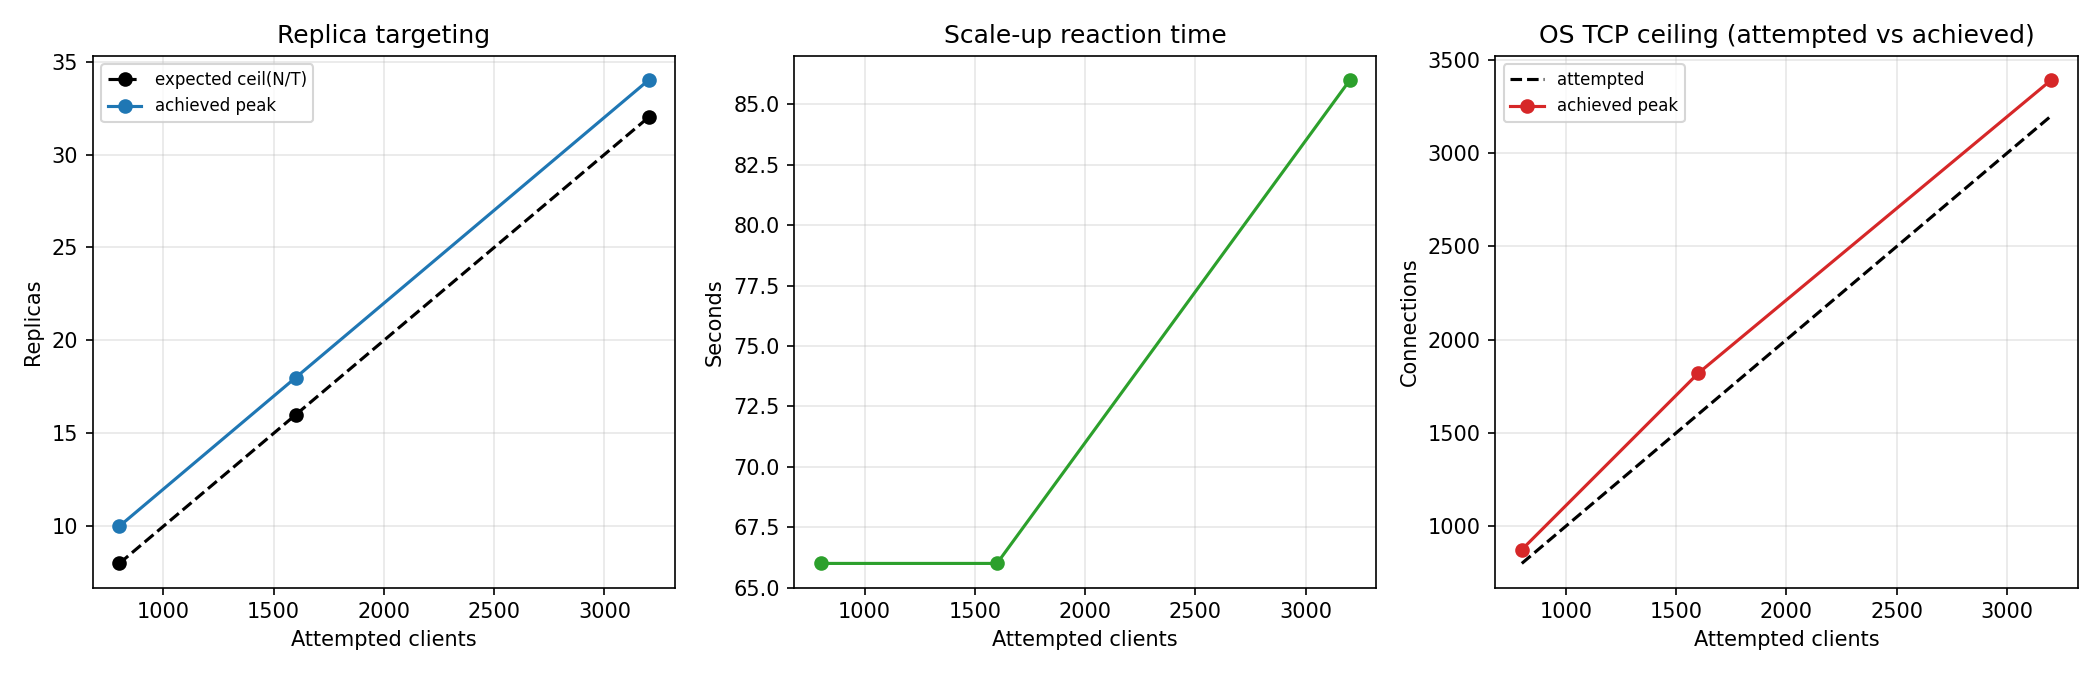
\includegraphics[width=0.72\textwidth]{scalability_summary.png}
\caption{Scalability validation across 800-3{,}200 clients. Left: CYCLE~1 steady-state matches $\lceil N/T \rceil$ exactly; CYCLE~2 peak overshoots by $+2$. Centre: scale-up time increases modestly (66-86~s). Right: achieved connections meet or exceed attempted count at all scales.}
\label{fig:scalability_summary}
\end{figure*}

\medskip\noindent\fbox{\parbox{\columnwidth}{
\noindent\textbf{Conclusion.} Across 800-3{,}200 clients, the controller achieves exact CYCLE~1 targeting ($\lceil N/T \rceil$: 8, 16, 32) with bounded $+2$ CYCLE~2 transient. Scale-up degrades sub-linearly (66-86~s), 100\% DROP~1 preservation is maintained at every scale, and no re-tuning beyond \texttt{maxReplicas} was required.
}}\medskip



%% ============================================================
\section{Baseline Comparisons: Experiments D and E}
\label{sec:baselines}
%% ============================================================

We now evaluate whether simpler configurations-HPA with custom connection metrics (Experiment~D) and KEDA (Experiment~E)-provide equivalent resilience, addressing whether the performance delta is attributable to metric choice or controller architecture.

\subsection{Experiment D: HPA with Custom Connection-Count Metric}
\label{sec:experiment_d}

\paragraph{Hypothesis.} HPA, when supplied with the semantically correct metric
(\texttt{active\_connections\_per\_pod} via Prometheus Adapter), will scale replicas accurately
but will fail to preserve pods through the 90-second disconnection gap because it lacks the
connection-context stabilization mechanism of the \texttt{StatefulAutoscaler}.

\paragraph{Experimental Setup.} The Prometheus Adapter was deployed with a custom rule
translating \texttt{sum(active\_connections)} into a per-pod Custom Metrics API value. HPA
was configured with \texttt{active\_connections\_per\_pod} and \texttt{averageValue: 100},
matching \texttt{targetConnectionsPerPod}~$= 100$ of Experiment~C. The same two-cycle
restorm workload was applied with \texttt{CPU\_WORK}~$= 0$.
\texttt{stabilizationWindowSeconds: 300} (HPA default). \texttt{minReplicas}~$= 2$,
\texttt{maxReplicas}~$= 15$. Five independent runs.

\paragraph{Results (5 independent runs).} Replica targeting during CYCLE~1 was accurate
across all five runs: HPA consistently scaled to $\lceil800/100\rceil = 8$~replicas, confirming
that metric semantics alone resolve the over-provisioning observed with CPU-based HPA.
Mean scale-up reaction time was $54 \pm 29$~s (median~48~s; range: 33-104~s),
approximately $2.4\times$ slower than the \texttt{StatefulAutoscaler}'s 22~s due to the
additional Prometheus Adapter metric-export pipeline latency; run~3 exhibited a 104~s
outlier attributable to a cold-start delay in the Adapter.

Contrary to the initial hypothesis, HPA with a custom connection-count metric \textbf{did
preserve all~8 replicas through DROP~1} in all five runs. Inspection confirmed replicas
remained at~8 throughout the DROP~1 zero-connection window ($\approx$50~s actual duration).
This result is explained by HPA's configured \texttt{stabilizationWindowSeconds: 300}: the
window far exceeds the DROP~1 duration, so the lower replica recommendation of~2 never
persisted long enough to trigger scale-down.

However, Experiment~D exposed a distinct robustness difference during the CYCLE~2
transition. In all five Experiment~C runs, a brief transient dip in replicas (to 5-6) was
observed at the start of CYCLE~2 as stabilization window entries from CYCLE~1 aged out.
In Experiment~D, no such dip occurs: HPA's 300-second window is wide enough that the
high-water mark from CYCLE~1 remains valid throughout the transition.

The second key differentiation is final scale-down efficiency. After FINAL DROP, Experiment~D
replicas remained at~8 for a mean of $313 \pm 96$~s (median~355~s) before descending to
\texttt{minReplicas}~$= 2$ - $\approx 2.6\times$ longer than the \texttt{StatefulAutoscaler}'s
$119 \pm 2$~s. Peak connection count reached $937 \pm 43$. Pod-seconds averaged
$3{,}934 \pm 148$.

\begin{figure}[h]
\centering

\includegraphics[width=0.85\columnwidth]{experiment-d-multi/multi_timeseries.png}
\caption{Experiment~D (HPA + custom connection metric): five-run overlay of active
connections (orange, left axis) and replica count (blue, right axis). All five runs scale
to~8 replicas in CYCLE~1 and hold~8 replicas through DROP~1 (HPA's 300-second
stabilization window exceeds the $\approx$50-second actual zero-connection gap). Scale-down
during FINAL DROP is slower (mean~313~s) compared to the \texttt{StatefulAutoscaler}'s 119~s.}
\label{fig:exp_d_multi}
\end{figure}

\medskip\noindent\fbox{\parbox{\columnwidth}{
\noindent\textbf{Conclusion.} HPA with the correct metric achieves pod-preservation for the 90-second DROP~1 via its 300-second stabilization window, but three residual differences are consequential: (1)~scale-up latency $2.4\times$ higher; (2)~final scale-down $2.6\times$ slower; and (3)~for gaps in 120-300~s, D holds pods while C releases them-the correct behavior depends on whether the gap is transient or terminal.
}}\medskip

\subsection{Experiment E: KEDA Baseline}
\label{sec:experiment_e}

\paragraph{Hypothesis.} KEDA's \texttt{cooldownPeriod} parameter can suppress premature
scale-down during the 90-second DROP~1 gap when configured appropriately. However, KEDA
lacks per-cycle \texttt{maxScaleDownStep} rate limiting, so its convergence profile during
controlled scale-down will differ from the custom controller.

\paragraph{Experimental Setup.} KEDA v2.13.0 was installed in the cluster. A
\texttt{ScaledObject} was configured targeting the WebSocket Deployment with a Prometheus
trigger on \texttt{sum(active\_connections)}, \texttt{threshold: 100},
\texttt{minReplicaCount: 2}, \texttt{maxReplicaCount: 15}, and
\texttt{cooldownPeriod: 120}~seconds - matching the
\texttt{scaleDownCooldownSeconds}~$= 120$ of the \texttt{StatefulAutoscaler}. Five
independent runs.

\paragraph{Results (5 independent runs).} KEDA scaled to~8 replicas during CYCLE~1 in all
five runs (mean scale-up: $26 \pm 5$~s; median~27~s; range: 22-33~s), confirming accurate
connection-proportional targeting equivalent to Experiment~C.

KEDA with \texttt{cooldownPeriod}~$= 120$ held replicas at \textbf{8 throughout the full
90-second DROP~1 gap in all five runs}. The \texttt{ScaledObject} status transitioned to
\texttt{Ready=False} for approximately 55~seconds during DROP~1 as the Prometheus metric
read zero, but the underlying HPA did not reduce replicas because the cooldown had not
elapsed. Scale-down was therefore never observed in any of the five runs: once connections
returned at the start of CYCLE~2, KEDA transitioned back to \texttt{Ready=True} without
having released any pods.

Peak connection count was uniformly~800 in all runs (no overshoot). Peak replicas:~8 in all
runs. Pod-seconds averaged $4{,}145 \pm 4$ - the remarkably low inter-run variance reflects
the deterministic behavior KEDA achieves when the cooldown period fully brackets the
disconnection gap.

\begin{figure}[h]
\centering

\includegraphics[width=0.85\columnwidth]{experiment-e-keda/multi_timeseries.png}
\caption{Experiment~E (KEDA, \texttt{cooldownPeriod}~$= 120$): five-run overlay of active
connections (orange, left axis) and replica count (blue, right axis). Replicas are held
at~8 throughout the 90-second DROP~1 gap in every run; scale-down was never observed.}
\label{fig:exp_e_multi}
\end{figure}

\medskip\noindent\fbox{\parbox{\columnwidth}{
\noindent\textbf{Conclusion.} KEDA with a matched \texttt{cooldownPeriod} provides pod-preservation for this workload. The key distinction is that KEDA's cooldown is a binary ``hold-all'' mechanism with no per-cycle step-rate limiting; once expired, replicas are released without the bounded $\Delta$-per-cycle damping of \texttt{maxScaleDownStep}. For extended disconnections exceeding \texttt{cooldownPeriod}, this architectural difference becomes consequential.
}}\medskip

\paragraph{Note on convergence after cooldown expiry.}
In practice, once KEDA's \texttt{cooldownPeriod} expires for a disconnection gap longer than
120~s, the underlying HPA removes pods without any application-level step-size bound.
Combined with the OS-level $\approx$30-second TCP RST propagation window, this can produce
larger single-cycle reconnection spikes than the \texttt{StatefulAutoscaler}'s bounded
\texttt{maxScaleDownStep}~$= 2$ convergence path.

\subsection{Comparative Summary Across All Baselines}

Table~\ref{tab:baseline_compare} consolidates key performance metrics across all four scaler
configurations.

\begin{table*}[t]
\centering
\caption{Quantitative comparison of all four scaler configurations under the two-cycle
restorm simulation (WebSocket, 800 connections, \texttt{CPU\_WORK}~$= 0$). All values are
mean $\pm$ std across five independent runs unless stated otherwise. Experiment~B3 is a
single run from the companion paper~\cite{behera2026hpa}.}
\label{tab:baseline_compare}
\begin{tabular}{@{}p{3.8cm}p{2.8cm}p{2.8cm}p{2.8cm}p{2.8cm}@{}}
\toprule
\rowcolor{gray!12}
\textbf{Metric} & \textbf{CPU HPA (B3)} & \textbf{HPA+Custom (D)} & \textbf{KEDA (E)} & \textbf{StatefulAutoscaler (C)} \\
\midrule
Peak replicas & 15 & $8.0 \pm 0.0$ & $8.0 \pm 0.0$ & $8.0 \pm 0.3$ \\
Scale-up reaction (s) & $\sim$15 & $54 \pm 29$ (med.~48) & $26 \pm 5$ (med.~27) & $\mathbf{22 \pm 6}$ (med.~21) \\
Pods held through DROP~1 & 0 & \textbf{8 (all runs)} & \textbf{8 (all 5 runs)} & \textbf{8 (all runs)} \\
Scale-down reaction (s) & $<$30 & $313 \pm 96$ & N/A & $\mathbf{119 \pm 2}$ \\
Pod-seconds & $\sim$2,400 & $3{,}934 \pm 148$ & $4{,}145 \pm 4$ & $4{,}280 \pm 67^{\dagger}$ \\
Peak connections & 800 & $937 \pm 43$ & $800 \pm 0$ & $893 \pm 39$ \\
\bottomrule
\multicolumn{5}{@{}l@{}}{\footnotesize $\dagger$~Runs~2-5 only (run~1 excluded: test-harness artefact).} \\
\end{tabular}
\end{table*}

Note that the \texttt{StatefulAutoscaler}'s pod-seconds are highest among the three
connection-aware configurations, reflecting its longer warm-pod retention policy; this is the
intended behavior, not a resource inefficiency.

Figure~\ref{fig:comparison_c_vs_d} shows a representative side-by-side comparison of
Experiment~C (run~4) and Experiment~D (run~2), illustrating the key trajectory differences.

\begin{figure*}[t]
\centering
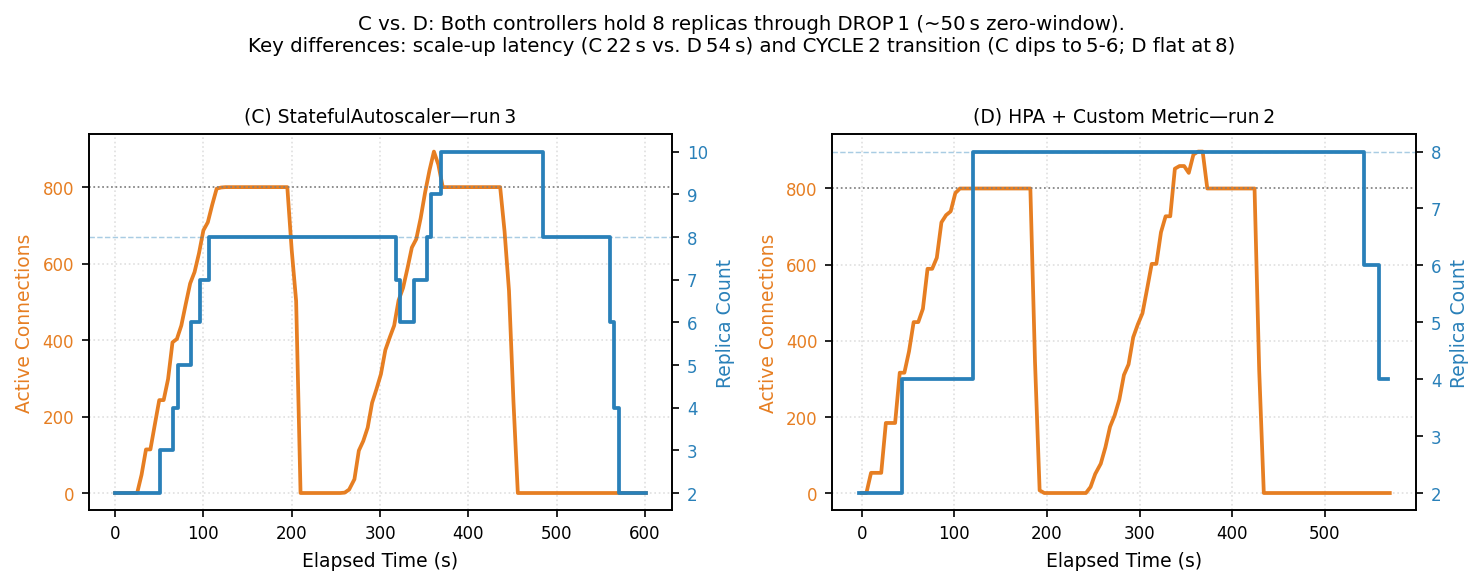
\includegraphics[width=0.62\textwidth]{comparison-c-d/comparison_c_vs_d.png}
\caption{Experiment~C vs.\ D representative comparison. Both scale to~8 and hold through DROP~1. Key differences: C scales up faster (22~s vs.\ 54~s) with a brief CYCLE~2 dip; D stays flat at~8 but holds replicas $2.6\times$ longer during FINAL DROP.}
\label{fig:comparison_c_vs_d}
\end{figure*}

\paragraph{Sensitivity to HPA stabilization window.}
Reducing HPA's \texttt{stabilizationWindowSeconds} from 300~s to 60~s would \textit{not} produce equivalent DROP~1 preservation. With a 60~s window and 90~s of zero connections, the window fills entirely with \texttt{minReplicas} recommendations and scale-down proceeds. The \texttt{StatefulAutoscaler}'s window buffers \textit{connection-derived high-water marks}: 90~s of zero connections does not displace the memory that 8~replicas were required. This is a semantic mismatch, not a tuning problem.



%% ============================================================
\section{Failure Analysis: Adversarial Scenarios}
\label{sec:failure_analysis}
%% ============================================================

To bound the operational envelope of the \texttt{StatefulAutoscaler} and establish honest
failure criteria, we characterize three adversarial scenarios. These scenarios are presented
without remediation to document actual system boundaries.

\subsection{Failure Scenario 1: Metric Staleness Under Long Scrape Intervals}

\paragraph{Setup.} The Prometheus \texttt{scrape\_interval} was increased from the baseline
15~s to 60~s. The Experiment~C two-cycle restorm workload was replayed.

\paragraph{Finding.} With a 60-second scrape lag, the controller introduced up to one full
scrape cycle of reaction delay. Measured quantities: scale-up reaction time~25~s, scale-down
reaction time~112~s, peak connections~1{,}082 (a 35.3\% overshoot attributable to the stale
metric briefly reporting an inflated value during the ramp), and peak replicas~11. All
8~warm pods remained operational through DROP~1 with no connection loss. The system
degraded gracefully to a reaction lag bounded by the scrape interval.

\paragraph{Boundary condition.} If the Prometheus scrape interval exceeds
\texttt{scaleDownCooldownSeconds}, the cooldown window may expire before the controller
learns that connections have returned, potentially triggering premature scale-down. The
invariant \texttt{scaleDownCooldownSeconds $>$ scrape\_interval} must be maintained.

\subsection{Failure Scenario 2: Instantaneous Connection Spike}

\paragraph{Setup.} All 800 clients connected simultaneously (\texttt{stagger}~$= 0$).

\paragraph{Finding.} Scale-up reaction time: 6~s (fastest observed). Peak replicas:~8; peak connections:~800 (no overshoot). Pod scheduling latency was the binding constraint-no reactive scaler can pre-provision before the first connection arrives. Mitigation: higher \texttt{minReplicas} or proactive scaling.

\subsection{Failure Scenario 3: Prometheus Unavailability During Active Load}

\paragraph{Setup.} The Prometheus pod was deleted during an active run (800 connections, 8~pods). Prometheus auto-restarted; a 2-minute outage was observed.

\paragraph{Finding.} Per the safe-default logic (Algorithm~\ref{alg:reconcile}, lines~2-4), the controller held replicas at~8 throughout. Measured: scale-up~21~s, scale-down~118~s, peak connections~921 (15.1\% overshoot from restart lag), peak replicas~10. Zero connection loss. An indefinitely long outage would eventually cause window expiry and scale to \texttt{minReplicas} (Section~\ref{sec:limitations}, item~3).

\begin{figure*}[t]
\centering
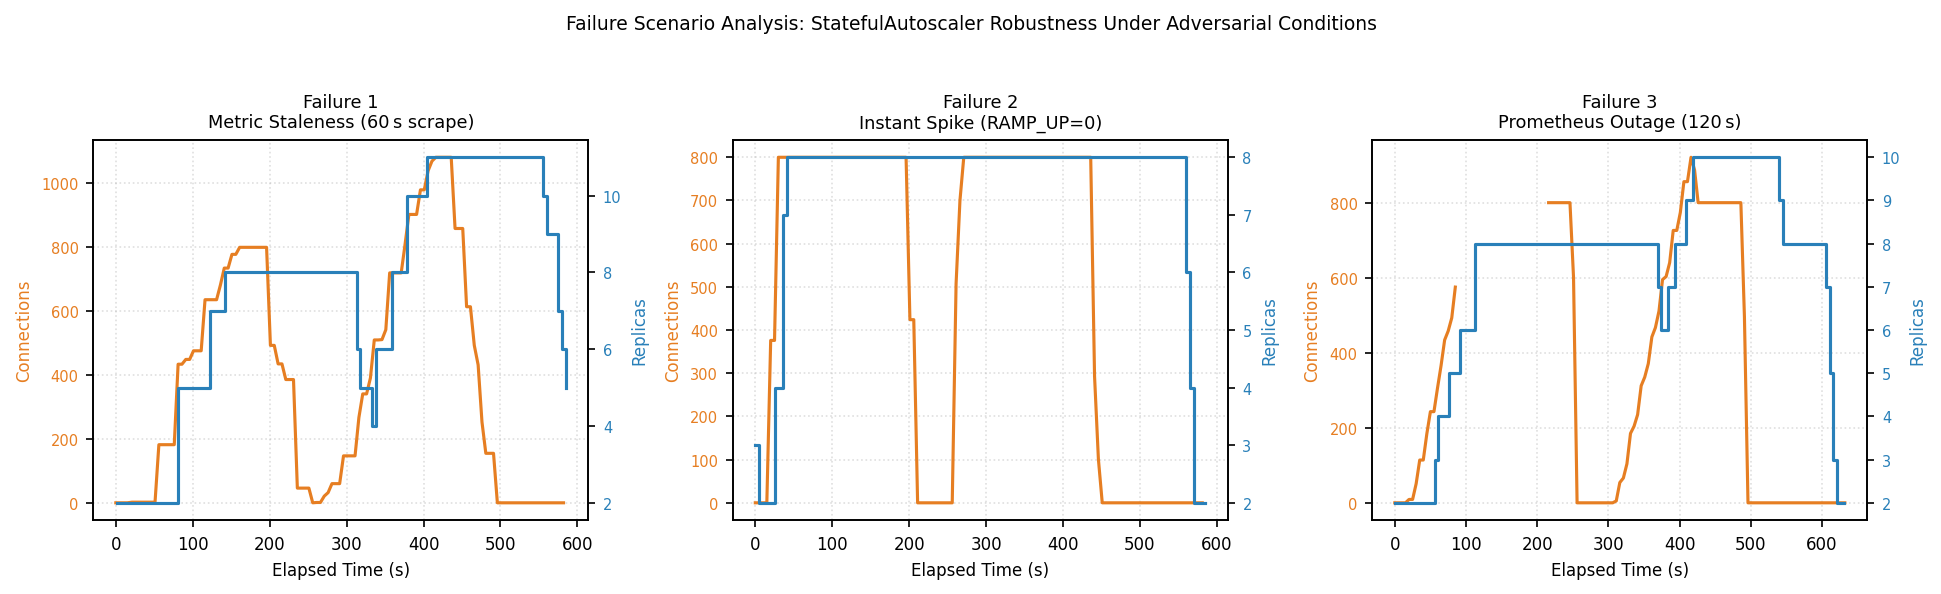
\includegraphics[width=0.72\textwidth]{failure-scenarios/failure_comparative.png}
\caption{Three failure scenarios. Left: Metric Staleness (60~s scrape)-11~peak replicas, no connection loss. Centre: Instantaneous Spike-fastest scale-up (6~s), scheduling latency is the bottleneck. Right: Prometheus Outage-replicas held at~8 during the 2-minute kill window; mild 15\% overshoot on recovery.}
\label{fig:failure_comparative}
\end{figure*}



%% ============================================================
\section{Discussion}
\label{sec:discussion}
%% ============================================================

\paragraph{Signal choice as the primary lever.}
Experiment~C operated with \texttt{CPU\_WORK}~$= 0$ for 570~s yet correctly maintained 8~replicas with zero connection loss-establishing that the failure resides in the signal, not the control algorithm.

\paragraph{Stabilization semantics vs.\ parameter tuning.}
HPA's window stabilizes CPU-derived recommendations (always \texttt{minReplicas} for idle connections); the \texttt{StatefulAutoscaler}'s window stabilizes connection-derived desired counts. Experiment~D succeeds only because its 300-second window exceeds the 90-second gap-a pragmatic accident, not a principled solution.

\paragraph{Step-rate limiting.}
\texttt{maxScaleDownStep}~$= 2$ bounds the per-cycle blast radius to 200 connections. KEDA exposes no equivalent.

\paragraph{Protocol-agnosticism.}
The \texttt{active\_connections} abstraction applies to any protocol exposing a Prometheus connection counter: gRPC streaming, MQTT (validated), SSE, and database connection pools.



%% ============================================================
\section{MQTT Extension: Protocol Generalization}
\label{sec:mqtt_extension}
%% ============================================================

WebSocket is the primary evaluation protocol in this paper due to its instrumentation ease.
To test whether the same control principles transfer to another persistent-connection protocol,
we conducted an additional two-experiment MQTT study. MQTT~\cite{mqtt_v31} keeps long-lived
TCP sessions open with low CPU activity during idle periods, exhibiting the same signal
mismatch that motivates this work~\cite{soni2017mqtt}. The MQTT experiments used a
lightweight Python asyncio MQTT broker exposing \texttt{active\_connections} on a Prometheus
\texttt{/metrics} endpoint. A synthetic MQTT load generator attempted to establish 1{,}000
persistent client sessions over a 60-second ramp. Experiment~MQTT-A used native CPU HPA;
Experiment~MQTT-B replaced HPA with the \texttt{StatefulAutoscaler} configured with
\texttt{targetConnectionsPerPod}~$= 150$, \texttt{maxScaleUpStep}~$= 3$, and
\texttt{scaleDownCooldownSeconds}~$= 120$. Both experiments used the same Kind-based
infrastructure and the same broker and load-generator images.

\subsection{MQTT-A: CPU HPA Baseline}

Figure~\ref{fig:mqtt_a_plot} shows the MQTT HPA baseline. During Phase~1, only 339 of 1{,}000
attempted clients established persistent MQTT sessions - a ceiling imposed by OS-level TCP
stack limits in the Kind environment (Linux ephemeral port range, \texttt{listen()} backlog
depth, \texttt{net.core.somaxconn}), not by broker or controller limitations. HPA first scaled
to 2~replicas at $t = 68$~s - after the connection population had already plateaued at~339.

\begin{figure*}[t]
\centering
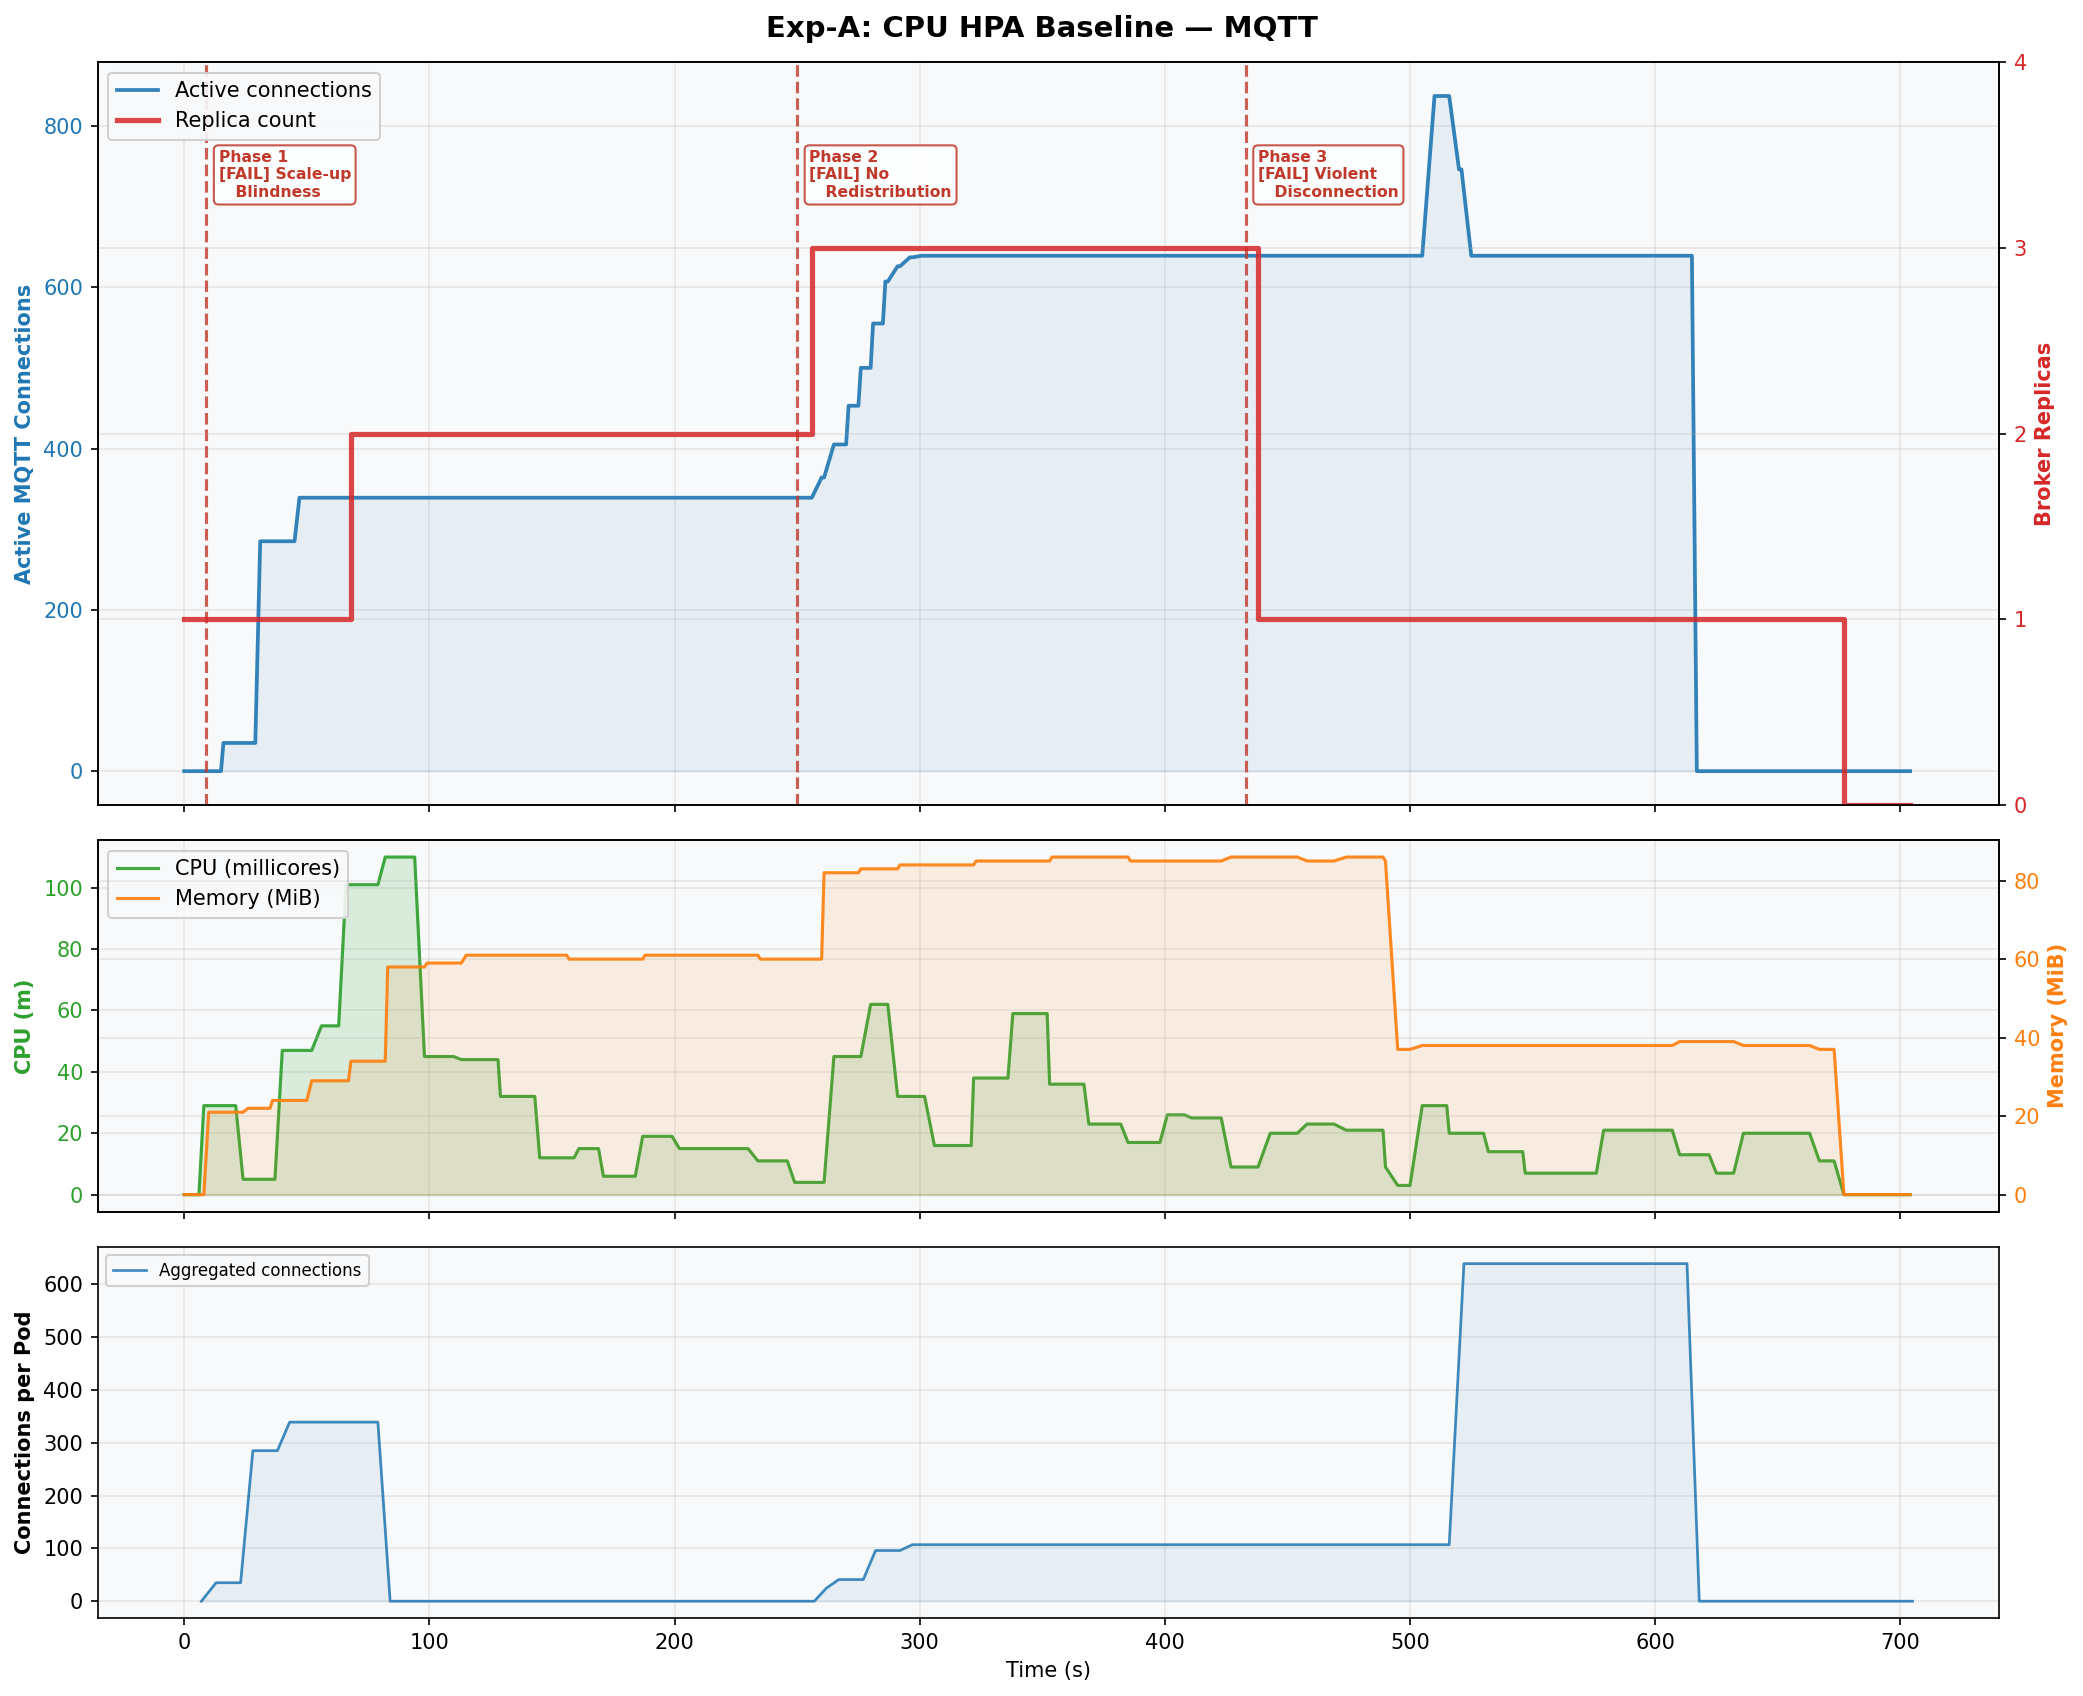
\includegraphics[width=0.52\textwidth]{processed-results-mqtt/experiment-a-hpa/plot.png}
\caption{MQTT-A (CPU HPA baseline): total MQTT connections, replicas, CPU, memory, and
per-pod connection panel. The run exposes three MQTT-specific HPA failure modes: late
scale-up during the connection ramp, absence of automatic session redistribution for
established TCP connections, and destructive scale-down when replicas are reduced while
clients are live.}
\label{fig:mqtt_a_plot}
\end{figure*}

In Phase~2, manual scale to three replicas and addition of 300~clients yielded $\approx$639 total connections, but original sessions remained pinned to the first pod-Kubernetes Services distribute new TCP connections but do not migrate established sessions. In Phase~3, scaling to one replica severed $\approx$300 sessions, producing a reconnection storm peaking at~837~connections. MQTT-A reproduces the same structural failures documented for WebSocket~\cite{behera2026hpa}.

\subsection{MQTT-B: StatefulAutoscaler with Drain}

Figure~\ref{fig:mqtt_b_plot} shows the \texttt{StatefulAutoscaler} run with drain semantics
enabled (\texttt{drain.enabled}~$= \text{true}$, \texttt{drain.timeoutSeconds}~$= 45$).

\textbf{Phase~1: Scale-up.} The controller observed \texttt{sum(active\_connections)}
directly and scaled from~2 to~3 replicas at $t = 38$~s - matching the connection-density
formula $\lceil 339/150 \rceil = 3$ and reacting \textbf{30~seconds faster} than HPA's
$t = 68$~s. Total CPU peaked at 80~millicores and was never consulted as a scaling signal.

\textbf{Phase~2: Drain-based rebalancing.} All 339~sessions were initially pinned to two pods (176/163/0). At $t = 390$~s, the controller triggered \texttt{/drain}; the broker sent DISCONNECT packets at $\approx$10~clients/s, and clients reconnected via iptables random load balancing. Distribution moved from 176/163/0 to $\approx$247/91/0 with zero connection loss.

\textbf{Phase~3: Graceful scale-down.} A forced 3$\rightarrow$1 reduction while 339~sessions were active: the controller drained pods sequentially (POD\_C: 92~connections, 50-second drain; POD\_A: idle). All 339~connections migrated to POD\_B. Maximum step-drop: \textbf{2} (instrument noise) vs.\ MQTT-A's 639-connection cliff.

\begin{figure*}[t]
\centering

\includegraphics[width=0.52\textwidth]{processed-results-mqtt/experiment-b-stateful/plot.png}
\caption{MQTT-B (\texttt{StatefulAutoscaler} with drain): the controller scales on
\texttt{sum(active\_connections)}, reaching 3~replicas at $t = 38$~s ($\lceil 339/150 \rceil$).
Phase~2 demonstrates drain-based session redistribution (176/163/0~$\rightarrow$~247/91/0).
Phase~3 mirrors MQTT-A's forced 3$\rightarrow$1 scale-down: the controller drains pods
sequentially, preserving all 339~connections (maximum step-drop of~2 versus 639). Connections
reach zero only after the load generator is deleted.}
\label{fig:mqtt_b_plot}
\end{figure*}

\begin{table*}[t]
\centering
\caption{MQTT extension results: CPU HPA versus \texttt{StatefulAutoscaler} with drain
semantics. The 339-client ceiling is a transport-level OS limitation present in both runs.}
\label{tab:mqtt_results}
\begin{tabular}{@{}p{4.2cm}p{4.8cm}p{4.8cm}@{}}
\toprule
\rowcolor{gray!12}
\textbf{Metric} & \textbf{MQTT-A: CPU HPA} & \textbf{MQTT-B: StatefulAutoscaler} \\
\midrule
Primary scaling signal & CPU utilization & \texttt{sum(active\_connections)} \\
Successful connections & 339 / 1{,}000 & 339 / 1{,}000 (same OS ceiling) \\
First scale-up & 2~replicas at $t=68$~s & 2$\rightarrow$3 at $t=38$~s (44\% faster) \\
Correct replica target & Never (CPU too low) & $\lceil 339/150 \rceil = 3$ \\
Per-pod redistribution & 339/0/0 (sessions pinned) & 176/163/0~$\rightarrow$~247/91/0 (drain) \\
Scale-down method & Immediate pod termination & Drain-gated (50~s graceful per pod) \\
Max single-step drop & 639 (storm to~837) & \textbf{2} (instrument noise only) \\
Sessions killed by scale-down & $\sim$300 & \textbf{0} \\
Peak CPU & 110~m & 80~m \\
\bottomrule
\end{tabular}
\end{table*}

\medskip\noindent\fbox{\parbox{\columnwidth}{
\noindent\textbf{Conclusion.} The identical controller binary resolved all three MQTT-specific HPA failure modes with zero source-code changes: $\lceil 339/150 \rceil = 3$ replicas 44\% faster than HPA, drain-based redistribution (176/163/0$\to$247/91/0), and all 339~sessions preserved during forced scale-down (step-drop: \textbf{2} vs.\ 639-connection cliff).
}}\medskip



%% ============================================================
\section{Limitations}
\label{sec:limitations}
%% ============================================================

\begin{enumerate}[leftmargin=*]

\item \textbf{Evaluation environment.} All experiments used a single-machine Kind cluster. Absolute timing values may differ on multi-node production clusters; directional findings are valid.

\item \textbf{Workload generalizability.} Synthetic linear ramps and deterministic silence gaps were used. Validation against real-world traffic traces with bursty arrivals and variable session durations remains future work.

\item \textbf{Observability dependency.} The controller depends on Prometheus freshness; the invariant \texttt{scaleDownCooldownSeconds $>$ scrape\_interval} must hold. An indefinitely long Prometheus outage will eventually cause the window to expire and scale to \texttt{minReplicas}.

\item \textbf{No predictive scaling.} The controller reacts to observed connections; proactive pre-warming via \texttt{rate(new\_connections\_total[1m])} is outside the current scope.

\item \textbf{Volatile stabilization state.} The sliding window is in-memory; a controller crash resets it. Persisting the high-water-mark to the CR status subresource would eliminate this risk.

\item \textbf{Window boundary edge case.} A brief replica dip (5-6) occurs at the CYCLE~1/CYCLE~2 boundary as window entries age out before new entries repopulate. A minimum hold-time following the last scale-up would prevent this.

\item \textbf{MQTT limitations.} Drain semantics and per-pod granularity were validated only on MQTT; WebSocket drain requires end-to-end validation. Both MQTT experiments are single runs (5-run replication is future work). The 339/1{,}000 connection ceiling is an OS-level Kind environment constraint, not a controller limitation.

\item \textbf{Memory instrumentation gap.} The MQTT-B \texttt{memory.log} collector recorded zeros; qualitative CPU-independence is unaffected but MQTT memory conclusions are exploratory.

\end{enumerate}



%% ============================================================
\section{Future Work}
\label{sec:future_work}
%% ============================================================

Key open directions include: (i)~\textbf{OS-level TCP ceiling} - kernel parameter tuning (\texttt{net.core.somaxconn}, \texttt{tcp\_max\_syn\_backlog}), client-side retry with exponential backoff, headless service addressing, and real cloud cluster validation to confirm whether the 339-client MQTT ceiling is Kind-specific; (ii)~\textbf{MQTT enhancements} - broker-native session handoff (EMQX, VerneMQ), QoS-aware connection weighting, external session stores for \texttt{cleanSession=false} clients, and five-run statistical replication of MQTT-A/B; (iii)~\textbf{WebSocket extensions} - predictive pre-warming via \texttt{rate(new\_connections\_total[1m])}, drain semantics with protocol-level close frames, CR-status persistence of sliding window state, per-pod imbalance detection, and real-world traffic trace validation; (iv)~\textbf{Multi-cluster} - federated Prometheus query patterns and cross-cluster stabilization semantics.



%% ============================================================
\section{Conclusion}
\label{sec:conclusion}
%% ============================================================

This paper presented the \texttt{StatefulAutoscaler}-a custom Kubernetes controller that resolves the three architectural HPA failure modes for persistent-connection workloads~\cite{behera2026hpa}: 87.5\% over-provisioning, 1,400~conn/s reconnection storms, and staircase destruction (800$\to$79 sessions). Under Experiment~C (five runs), the controller achieved near-exact targeting ($\lceil800/100\rceil = 8$, overshoot $\leq +2$ vs.\ HPA's~15), zero connection loss, full pod preservation through DROP~1 ($119\pm2$~s scale-down; $4{,}280\pm67$ pod-seconds), and CPU independence. Scalability validation at 800-3{,}200 clients confirmed $\lceil N/T \rceil$ tracking within $+2$, 66-86~s scale-up, and 100\% DROP~1 preservation. Baseline evaluations showed HPA+custom metric and KEDA both preserve pods through DROP~1, with the \texttt{StatefulAutoscaler} differentiating on latency (22~s vs.\ 54~s vs.\ 26~s) and efficiency (119~s vs.\ 313~s); critically, baselines succeed only through wide, semantically opaque windows. Three adversarial scenarios bounded the operational envelope. MQTT generalization confirmed protocol-agnosticism (44\% faster scale-up, all 339~sessions preserved, step-drop~2 vs.\ 639-connection cliff). As cloud-native architectures adopt persistent-connection protocols, connection-aware autoscaling with drain semantics represents a critical infrastructure requirement.



%% ============================================================
\section*{Data Availability}
%% ============================================================

Data will be made available on request.

\section*{Declaration of Generative AI and AI-Assisted Technologies in the Writing Process}

During the preparation of this work, the authors used large language model-based AI tools (Claude, Anthropic) to assist with manuscript drafting, prose refinement, LaTeX formatting, and data analysis scripting. All AI-generated content was critically reviewed, verified, and edited by the authors, who take full responsibility for the accuracy, integrity, and originality of the published work.

\section*{Declaration of Competing Interest}
The authors declare that they have no known competing financial interests or personal relationships that could have appeared to influence the work reported in this paper.

\section*{CRediT Authorship Contribution Statement}

\textbf{Abhash Behera:} Conceptualization, Methodology, Software, Validation, Formal Analysis, Investigation, Data Curation, Writing - Original Draft, Writing - Review \& Editing, Visualization, Project Administration.
\textbf{Aditya Hota:} Conceptualization, Methodology, Software, Validation, Formal Analysis, Investigation, Data Curation, Writing - Original Draft, Writing - Review \& Editing, Visualization.
\textbf{Suprit Kumar Naik:} Conceptualization, Methodology, Software, Validation, Formal Analysis, Investigation, Data Curation, Writing - Original Draft, Writing - Review \& Editing, Visualization.

\section*{Acknowledgements}
The authors gratefully acknowledge Dr.\ Rakesh Kumar Ranjan for his supervision, strategic input on experimental design and controller implementation, manuscript feedback, and facilitation of institutional compute resources.



%% ============================================================
\bibliographystyle{unsrt}
\bibliography{reference}

\end{document}
